\documentclass[english, a4paper, 12pt]{article}
\usepackage{multirow,booktabs}
\usepackage{appendix}
\usepackage{times}
\usepackage{siunitx}
\usepackage{tabularx,booktabs}
\usepackage{bm}
\usepackage{subfig}
\usepackage{geometry}
\usepackage[hidelinks]{hyperref}
\usepackage{pdfpages}
\usepackage{footnote}
\usepackage{graphicx}
\usepackage{rotating}
\usepackage{amsmath}



\usepackage{listings}
\usepackage{color} %red, green, blue, yellow, cyan, magenta, black, white
\definecolor{mygreen}{RGB}{28,172,0} % color values Red, Green, Blue
\definecolor{mylilas}{RGB}{170,55,241}


\makeatletter
\renewcommand{\section}{\@startsection
{section}%                   % the name
{1}%                         % the level
{0mm}%                       % the indent
{-1.5\baselineskip}%            % the before skip
{0.5\baselineskip}%          % the after skip
{\normalfont\Large\bfseries}} % the style
\makeatother

\usepackage{listings}
\lstset{
    language=Matlab,
    basicstyle=\footnotesize\ttfamily,
    columns=flexible,
    keepspaces=true,
    keywordstyle=\color{red},
    commentstyle=\color{blue},
    breaklines=true,
    tabsize=2
}

\newcommand\abs[1]{\left|#1\right|}
\newcommand{\at}{\makeatletter @\makeatother}	
\newcommand{\grader}{$^\circ$}
\newcommand{\medf}{\qquad\Leftrightarrow}
	
\newcommand{\x}{\mathbf{x}}	
\newcommand{\A}{\mathbf{A}}	
\newcommand{\B}{\mathbf{B}}	
\newcommand{\C}{\mathbf{C}}	

% Winning
\newcommand\mat[1]{\mathbf{#1}}
\newcommand{\trans}{^\mathsf{T}}

\lstset{language=Java,%
    %basicstyle=\color{red},
    breaklines=true,%
    morekeywords={matlab2tikz},
    keywordstyle=\color{blue},%
    morekeywords=[2]{1}, keywordstyle=[2]{\color{black}},
    identifierstyle=\color{black},%
    stringstyle=\color{mylilas},
    commentstyle=\color{mygreen},%
    showstringspaces=false,%without this there will be a symbol in the places where there is a space
    numbers=left,%
    numberstyle={\tiny \color{black}},% size of the numbers
    numbersep=9pt, % this defines how far the numbers are from the text
    emph=[1]{for,end,break},emphstyle=[1]\color{red}, %some words to emphasise
}

\renewcommand{\thesubsection}{\thesection.\alph{subsection}}
%\renewcommand{\thesubsection}{\alph{subsection})}


%==============================================================>

\begin{document}


\includepdf{figures/Frontpage.pdf}

\section{Introduction}

\subsection{Introduction to Web services}
\paragraph{Description of Web services}
A web service is a way to send messages between applications over a network.

\paragraph{Service orientation}
This is a very service orientated project. This statement is based on the fact that every bit of functionality was implemented to satisfy the demand of a service specified in the problem description. In order to implement the functionality these services require, we are making use of several web service technologies.
Basic service technologies

\paragraph{XML}
XML is a markup language for encoding documents. Probably the greatest advantage of XML syntax is that of simplicity; it is easily read- and writeable for humans.

\paragraph{SOAP}
SOAP is a protocol for exchanging messages between web services. The document format of SOAP messages is written in XML. The most notable advantage of SOAP is its versatility. SOAP can use any transport protocol and allows for any programming paradigm. SOAP was initially required to use HTTP as transmission protocol.

\paragraph{WSDL}
WSDL is a language for describing the functionality of web services and how to access these. A WSDL document can basically be thought of as an interface to a web service. Like SOAP WSDL is written in XML resulting in a high degree of readability.
Web service discovery
For web service discovery we use WSIL, which basically revolves around asking a web service provider what services it provides in order to discover these. The services are then described in WSDL format.

\paragraph{Web service composition}
Web service composition is the act of combining services into more powerful business processes. Client requests cannot always be satisfied through the use of a single service. Therefore, service composition is used to create one service with all the required operations.
Web service coordination
Web service coordination is when a number of web services need to coordinate to complete a goal and thus, it is the process of making them coordinate. A coordinator combines operations that are used to complete the same goal, and checks these operations by sending information to make sure they have done their part.

\paragraph{BPEL}
BPEL is a language for writing web services in the shape of business processes. It is based on XML.
A BPEL process consists of at least one activity. The most relevant basic activities are invoke, receive, assign and reply.
The invoke activity calls a partner web service. The receive activity functions as an entry point to a web service and the reply activity is then used for sending a response with some data to the previous web service. Assign activities can be used in between to assign values to the data fields, which are to be returned.
Partner web services are defined using partnerlinks specifying the role and type of the partner.

\paragraph{RESTful services}
RESTful web services function stateless and only use the HTTP verbs: GET, POST, PUT and DELETE. This means that no information about the client is being stored on the server. The limitation of only four operations helps make REST a simple web architecture.
GET requests information.
POST is used for sending information.
PUT replaces old information with new information.
DELETE deletes information.

\paragraph{Security}
Security has not been a focus point for our work and therefore the application and its services will not prevent users from doing most unauthorized operations.



\section{Coordination Protocol}
The user will interact solely with a composite webservice running either as a BPEL program or a RESTful process. This interaction should involve no data parsing on the client side, thus allowing for a simple and elegant user experience. All data parsing, storage and general orchestration of the business process will occur in the composite webservice. The user is considered to be well-behaved, meaning that all input given by the user fits the data types and representations described in the schema files. 

A user will initiate the business process by calling the “StartItinerary” function of the composite webservice. The composite webservice will assign a globally unique identifier to the new customer, and return said identifier to the user. The user must now provide this identifier whenever he or she wishes to communicate with the composite webservice. 

Once an itinerary has been created, the user is free to request flights and hotels, add flights and hotels to the itinerary, cancel the itinerary or book added flights and hotels.
In order to add items to the itinerary, the user must first obtain valid representations of the flights or hotels that he or she wishes to add. In this case, the composite webservice functions as a proxy to the services provided by NiceView and LameDuck, piping the parameters provided by the user to the remote service, and returning the corresponding return value to the user. The user can then choose suitable flights or hotels and add them to the itinerary.

The user may request a representation of the itinerary at any time. Only at the time of the first flight, or upon cancellation of an unbooked itinerary, will the resources occupied by the business process be released.

When the booking of an itinerary is attempted, the composite webservice will report whether all bookings were successful. In the event that a booking fails, the user will be notified by a false return value and may prompt the composite webservice for his or her itinerary to inspect the details of the problematic operation. The same is the case when attempting to cancel an itinerary.

Once and itinerary has been booked, the user is no longer allowed to query for flights and hotels or add new flights and hotels to the itinerary. At this point, the only operations that may be carried out are the ones associated with getting the itinerary and cancelling it.

The sequence diagram shown in figure \ref{fig:sequence} depicts the interactions of a user with the composite webservice. As shown in the diagram, the TravelGood service is responsble for coordinating the activities of the user with those of other services, i.e. NiceView. The portrayed scenario involves the creation of an itinerary, the querying of hotels by way of NiceView, the addition of a hotel to the itinerary and finally the booking and retrieval of the final itinerary. The interactions of the different webservices have been simplified to provide a more intuitive diagram.

\begin{figure}[h!]
\centering
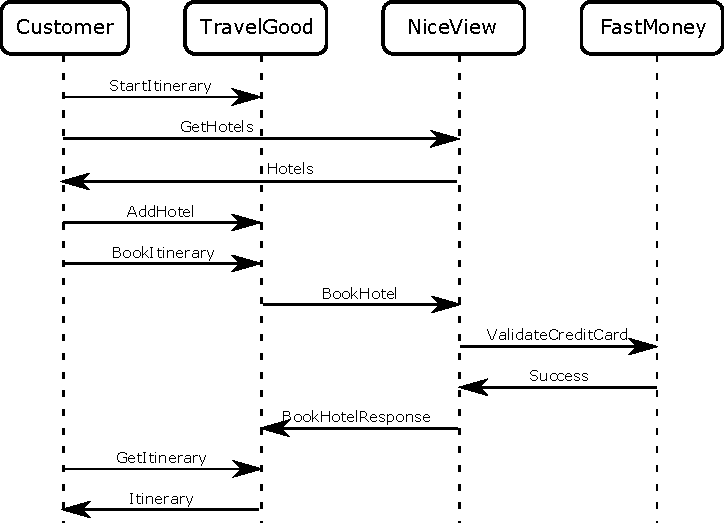
\includegraphics[width=0.9\textwidth]{figures/SequenceDiagram.pdf}
\caption{Example of sequence of user interactions}
\label{fig:sequence}
\end{figure}



\section{Web service implementations}


\subsection{A section on the data structures used}


\subsection{Airline- and Hotel Reservation Services}
The Airline service LameDuck is a simple SOAP-based web service that allow users to list, book and cancel flights. The service has three corresponding methods: getFlights(), bookFlight(), and cancelFlight(). The getFlights method returns an array of the complex type FlightInfo containing all the relevant information about a single flight. The list can be empty, if no flights are found. These flights can be booked or cancelled. If anything goes wrong, or the user provides invalid inputs, a FlightFaultMessage exception will be thrown. 

The hotel booking service NiceView is very similar to LameDuck, and has the same three functions: get, book, and cancel. When an error occur, the HotelFaultMessage exception is thrown. When getHotels is called, a list of the complex type HotelInfo is returned.

The two simple web services are implemented in a top-down fashion with document-style bindings and a literal use. The document/literal style WSDL is advantageous since ( Todo: )

Developing the web service top down means writing the WSDL file first, and then generating java classes representing the service. In a bottom up development, you would write the Java classes first, and then generate the WSDL file. The top-down approach is preferred, since it ensures that the WSDL file is exactly as you want it to be, and that it remains constant even if the Java code is changed. The WSDL file is a contract between the server and the client, which tells the client how to interface with the server. Whenever the WSDL file changes, the contract is “violated”, and  every client must be notified of this change, and they have to modify their code. Using a bottom up approach might lead to changing WSDL files, even when minor changes are made. Different toolchains can generate different WSDL files from the same code, so if the tool is updated, it can result in a changed WSDL file.

\subsection{Business Process Implementation Using BPEL}
Our BPEL process is a process of collaboration between the client and the web services using partnerlinks. The message flow works by invoking operations defined in WSDL files for the two webservices: LameDuck and NiceView. These WSDL files are made by hand and are not generated from Java classes. Furthermore, the client itself is a WSDL file consisting of messages with parts as well as operations. Using the basic activities we’ve mentioned in the introduction, such as receive, invoke, assign and reply, we exchange messages between the client and the services.

There are three port types across the BPEL implementation, TravelGood, LameDuck and NiceView. These each define the operations and messages for the respective web service they define. We’ve designed the system this way to keep the different operations separate as the assignment requires, and because it would not make sense to have the two reservation services together. 
For binding style we have chosen document. This design choice is due to the fact that we exchange a lot of messages between the various services, and we would like to have control over these request and response messages. The literal encoding, as opposed to the encoded encoding, is a result of the schemas we define in the WSDL files. With document/encoded, we would have no schemas, which wouldn’t make sense.

The BPEL process starts with a startItinerary operation to initiate the process. We use several structured activities to keep the process going, so that the process can continue instead of ending after every operation. Using a pick activity we redirect the flow to other sequences based on the message received. This way the client can choose which operation to execute instead of having to go through several unnecessary operations. We have illustrated tis initial design decision in section 2, Coordination protocol. All of these choices are wrapped in a while activity to keep the process going. Furthermore, some sequences are wrapped in if-activities to check whether the client has finished adding hotels etc. This allows the client to keep adding instances of bookings. Additionally, the BPEL process also contains fault handlers to catch possible faults. These include the logic to, for example, cancel hotels and flights, should Itinerary booking fail.

\subsection{Business Process Implementation Using RESTful}
There are three resources: ItineraryResource, FlightsResource and HotelsResource. FlightsResource and HotelsResource have only GET methods for serving fetching hotels/flights from web services. ItineraryResource has POST: addItinerary (for adding itinerary; because it is new entry); GET: getCurrentItineraries, getItinerary (for fetching list of itineraries by user, and just one itinerary); PUT: addHotel, addFlight, bookItinerary (for adding hotels/flights and booking itinirary; because we already have entry and now modifying it); DELETE: deleteHotel, deleteFlight, cancelPlanning (removing hotels/flights from itinerary and canceling it).

We rejected idea when in resource hotel/flight there are POST, DELETE, because it is not creation of new hotel/flight and removing it, it all about managing data structure Itinerary, serving lists inside of it.

Besides resources our REST has three other namespaces: helpers (consist of wrappers for each data type for proper output in XML/JSON), structures (has Itinerary data structure) and services (communicate with web services).

Structures of flights/hotels are imported using web service references, and Itinerary is stored inside REST, it consist of: id, hotelBookingList, flightBookingList, currentStatus and closestDate.

There are three services; all of them made in singleton style; structure of FlightsService/HotelsService have imported functions from web services and public functions for using them; in ItineraryService we have HashMap<String, Itinerary>, which make search for edition and reading faster, we use itineraries.get(id); also we transfer all the time userId and check if user has access to the entry. 



\section{Web service discovery}
%Create three WSIL les, one for each company (TravelGood, LameDuck, and NiceView). Each WSIL file should link to each other WSIL file. Each WSIL should contain references and descriptions of the Web services offered by each company as defined in Sect. 2.3.

\section{Comparison RESTful and SOAP/BPEL Web Services}
\section{Advanced Web service technology}
\paragraph{WS-Addressing}
WS-Addressing works by sending information about who sent a SOAP message and information about the recipient in the header of the SOAP message.

See WS-Security for discussion of the possible benefits of identification information.

\paragraph{WS-Reliable Messaging}
As the name indicates the idea of WS-Reliable Messaging is to make the transmission of SOAP messages from A to B more reliable. This is accomplished using acknowledgement messages. The recipient B sends acknowledgement messages for each message received back to A. Based on these acknowledgements A will know which messages to resend in order for B to have received all of the messages. This ensures that messages are retransmitted to B until acknowledged, and makes it possible for A to have the messages arrive in order.

When calling one-way services, ACK messages are very beneficial because otherwise you might not have a way to know whether the message was received or not. Regarding request-response services the usefulness of acknowledgements depends on the timeout for the sent message. If the message activates a time consuming service, the timeout would have to be equally long to ensure a timeout does not occur, before the service is finished and has responded.
Therefore it will not be particularly beneficial for our web services to make use acknowledgement messages, since we use request-response services with relatively short processing time.

\paragraph{WS-Security}
WS-Security attempts to ensure 3 things: Sender identity, message integrity and message confidentiality. It does so using mainly security tokens, digital signature and encryption.

As the customer books flights and hotels and fills the itinerary, WS-Security can help ensure that we are in fact receiving requests from the same customer who started the itinerary.
It will also be beneficial to ensure the integrity of the messages, so that as an example an attacker cannot have the customer pay for flights for another person.
Our services handling delicate information such as credit card information would benefit greatly from encryption. This will help ensure that third parties cannot read the information if they monitor the message exchange.

\paragraph{WS-Policy}
WS-Policy allows for specifying rules web services have to follow. In order to do this WS-Policy makes use of assertions to set up boolean expressions and thereby check if the rules have been met. WS-Policy can with advantage be used for configuring WS-Security and WS-Reliable Messaging.



\section{Conclusion}
%This section should summarise the report and contain the experiences with the project. For example, what was learned, what are the things you can improve next time, and what did made good this time. (Won't be graded!)


\section{Who did what}






\end{document}
